\chapter{Systèmes de mesure}

\section{Introduction}

Les mesures comme celle de la température, de l'heure ou de notre masse corporelle sont des activités quotidiennes si courantes que l'on porte généralement peu d'attention à l'instrument de mesure et à l'exactitude du résultat.

Pour des équipements plus complexes, comme ceux que l'on trouve dans les installations scientifiques, industrielles, et médicales, l'exactitude de la mesure revêt en revanche un aspect critique, essentiel. Il peut être en effet nécessaire de respecter des normes, de garantir la fiabilité d'un composant, de vérifier une prédiction théorique: on doit donc être assuré de la \textbf{qualité des mesures} que l'on effectue. Pour cela il est indispensable d'apporter une grande attention à l'instrument de mesure ainsi qu'à la façon dont celle-ci est effectuée.

Un système de mesure est généralement constitué de quatre parties (fig.~\ref{fig:sysmes}):
\begin{description}
    \item[le capteur] qui traduit la valeur physique mesurée en un signal; il utilise un phénomène physique réagissant à la grandeur à mesurer et assure sa transformation en un signal électrique, optique ou mécanique plus facile à manipuler et à quantifier (voir le cours HEIG-VD \textit{capteurs}).
    \item[le conditionneur] qui transforme le signal pour le mettre dans une forme adéquate à sa lecture - par exemple l'amplifier ou le filtrer,
    \item[la sortie] de l'instrument de mesure qui permet de lire puis enregistrer la mesure,
    \item[un système de contrôle (optionnel)] par feedback dans le cas où le système de mesure est inclus dans un contrôle de processus.
\end{description}
\begin{sidewaysfigure}[p]
    \centering
    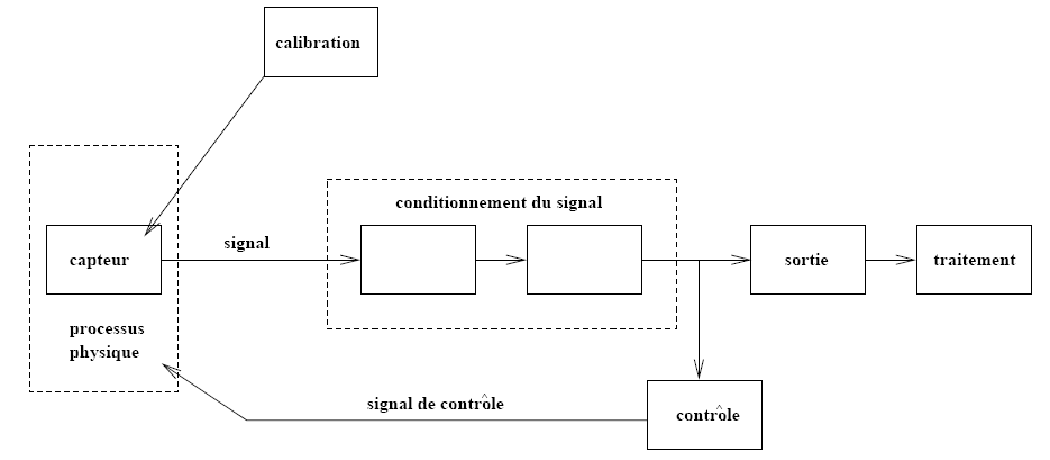
\includegraphics[width=20cm]{assets/figures/systemeMesure.pdf}
    \caption{Schéma général d'un système de mesure}
    \label{fig:sysmes}
\end{sidewaysfigure}

\section{Les différents types de signaux}

Un système de mesure transforme une \textbf{entrée}, en règle générale une grandeur physique, en un signal de \textbf{sortie}. différents types de signaux sont transmis entre les capteurs, les conditionneurs et la sortie du système.

On peut classifier les signaux en trois catégories selon leur représentation temporelle et les valeurs prises par la quantité mesurée (fig.~\ref{fig:typsign}):
\begin{description}
    \item[Un signal continu] est défini pour toutes les valeurs du temps et peut prendre n'importe quelle valeur en amplitude,
    \item[Un signal discret] est en général un signal continu qui est mesuré à certains instants seulement, mais il peut aussi s'agir d'un signal naturellement discontinu, tel que le nombre de photons reçus par un détecteur pendant une certaine durée de temps, un nombre de véhicules par tranche d'heure sur une route, etc.
    \item[Un signal numérique] est un signal discret quantifié sur un certain nombre de niveaux (généralement des puissances de 2) et qui ne peut prendre qu'un ensemble discret de valeurs, par exemple la numérisation d'un signal électrique de -10 à +10 V sur 8 bits non signés, de 0 à 255.
\end{description}
\begin{figure}[h]
    \centering
    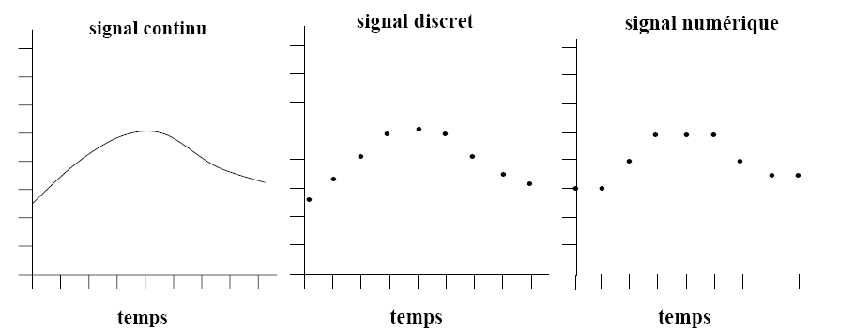
\includegraphics[width=16cm]{assets/figures/typesign.pdf}
    \caption{Les trois types de signaux les plus fréquents.}\vspace{5mm}
    \label{fig:typsign}
\end{figure}

\newpage
En fonction du phénomène physique qu'ils représentent, il faut aussi distinguer les signaux \textbf{déterministes}, c'est-à-dire les signaux pour lesquels les valeurs futures peuvent être prédites, et les signaux \textbf{aléatoires} qui ne sont pas prédictibles et qui nécessitent un traitement spécifique (fig.~\ref{fig:sigda}).
\begin{figure}[h]
    \centering
    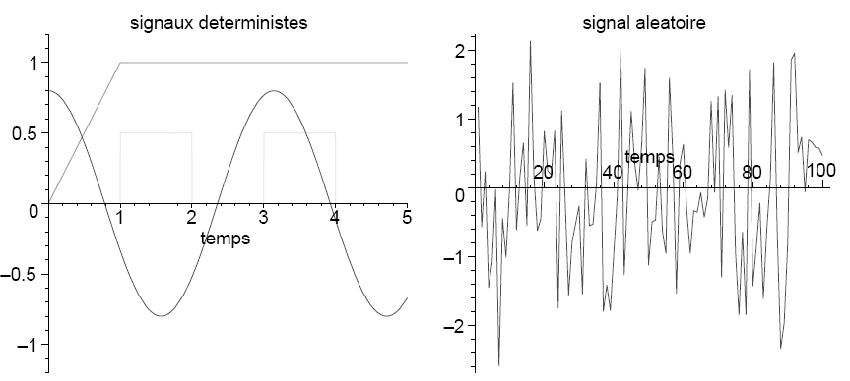
\includegraphics[width=16cm]{assets/figures/sigda.pdf}
    \caption{Signaux déterministes et aléatoires.}
    \label{fig:sigda}
\end{figure}

\section{méthodes générales de mesure}

\subsection{Mesure par déviation}

C'est la méthode qui consiste à obtenir la déviation d'un système, d'une position d'équilibre qu'il occupait en l'absence de mesurande, à une nouvelle position d'équilibre qu'il occupe en présence du mesurande.  L'écart entre les deux positions fournit plus ou moins directement la mesure.

Dans la méthode de déviation par \textbf{élongation simple}, les deux positions sont des positions au sens géométrique du mot; elles ne mettent pas en jeu un équilibre particulier de force. Ainsi en est-il de la mesure d'une longueur au pied à coulisse, oà l'opérateur déplace les palpeurs pour venir en contact entre eux (zéro), ou sur la pièce (mesure).

Dans la méthode de déviation par \textbf{équilibre spontané}, les positions d'équilibre sont le résultat d'une opposition entre deux forces égales. L'exemple typique d'une mesure par \begin{wrapfigure}[13]{r}[0pt]{3cm}
    \centering
    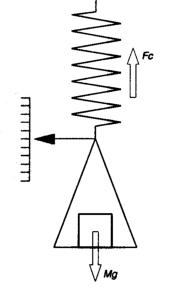
\includegraphics[width=3cm]{assets/figures/mesdev.pdf}
    %   \caption{Peson à ressort}
    %   \label{fig:mesdev}
\end{wrapfigure}
équilibre spontané est le \textbf{peson à ressort} (figure ci-contre). On suspend une masse sur un plateau fixé à l'extrémité d'un ressort vertical. Les forces de résistance, dont le ressort devient le siège quand il est déformé, et est proportionnel à l'allongement, augmentent jusqu'à égaler le poids du corps, et c'est la valeur de l'allongement du ressort, à l'équilibre, qui indique la masse. On peut certes calculer les forces développées à partir des caractéristiques du ressort, mais il est plus simple et plus précis de tarer le ressort avec des masses connues.

Les appareils qui utilisent la méthode de déviation sont innombrables en métrologie. Quelques types élémentaires sont mentionnés dans le tableau ci-dessous:
\begin{center}
    \begin{tabular}{llll}
        Appareil            & Mesurande   & Grandeur d'opposition  & Mesure                  \\ \hline
        Peson à ressort     & force       & contrainte ressort     & allongement             \\
        Peson à contrepoids & force       & moment d'une force     & angle                   \\
        Baromètre à mercure & pression    & pression hydrostatique & différence de niveau    \\
        Thermomètre à gaz   & température & volume                 & déplacement d'un niveau
    \end{tabular}
\end{center}

\vspace{4mm}
Le \textbf{galvanomètre} à cadre mobile (figure \ref{fig:galva}) est un autre exemple de méthode par déviation. C'est l'égalité du couple produit par les forces électromagnétiques et du contre-couple généré par la torsion du fil de suspension du cadre qui définit la déviation qui donne la mesure. Le système se déforme jusqu'à ce que cet équilibre soit atteint.
\begin{figure}[h]
    \centering
    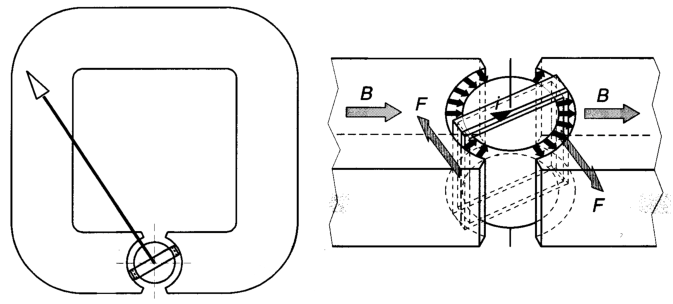
\includegraphics[height=4.6cm]{assets/figures/galva.pdf}
    \caption{Principe du galvanomètre. À gauche, on observe l'aimant permanent générateur d'un champ magnétique à travers le cadre mobile du galvanomètre. À droite, vue détaillée du cadre et de la force d'origine électromagnétique subie par le cadre dans lequel circule le courant (ou la tension) que l'on désire mesurer.}
    \label{fig:galva}
\end{figure}

Dans ce cas, cependant, la transformation et transmission d'énergie sont moins directes que dans le cas du peson: le premier effet de la tension électrique appliquée aux bornes du cadre sera d'instaurer un courant continu qui dépend des constantes électriques du circuit. Ce courant, plongé dans le champ magnétique de l'aimant permanent, crée une force électromagnétique mettant en rotation le cadre, et partant, tord le fil de torsion, support du cadre. Le contre-couple dé à la torsion du fil augmente avec l'angle de rotation du cadre, jusqu'à se trouver en équilibre et compenser le couple engendré par la force électromagnétique. La rotation est alors stabilisée, et après quelques instants d'oscillation, la valeur finale pourra être lue.

\subsubsection{précautions d'emploi de la méthode par déviation}

Mentionnons quelques précautions exigées par l'emploi de la méthode par déviation :
\begin{itemize}
    \item\textbf{Mise à zéro} : la mesure est fournie par l'écart à partir d'une position d'origine prise comme zéro. Il est donc impératif de vérifier que l'instrument indique effectivement zéro en l'absence de mesurande. Sinon il faudra noter la position de départ qui est un "faux zéro". Les instruments électroniques, les thermomètres, les manomètres présentent souvent des décalages de zéro (en anglais \textit{offset}) dont il faut tenir compte.
    \item Il faut attendre que l'\textbf{équilibre soit atteint}.
    \item Il faut aussi porter attention aux \textbf{conditions de linéarité}: en effet, la loi la plus avantageuse qui puisse relier le mesurande et la mesure, tant pour son interprétation immédiate que pour son traitement ultérieur, est une \textbf{relation linéaire}. C'est elle que l'on cherche généralement à obtenir. Un bon moyen d'y parvenir est de n'utiliser que des transducteurs\footnote{Un transducteur est un dispositif convertissant un signal physique en un autre; par exemple un signal lumineux en signale nerveux (vision animale) ou signal électrique (photorécepteur).} linéaires dans la chaîne de mesurage. Les transducteurs sont en général linéaires dans une plage plus ou moins étroite de l'étendue, généralement au voisinage du zéro. Si le système de mesure comporte un traitement numérique, il est possible d'introduire, dans le programme traitant les mesures, la courbe de calibration du capteur, ce qui élimine les problèmes de non-linéarité.
\end{itemize}

\newpage

\subsection{Mesure par comparaison}

\begin{wrapfigure}[10]{l}[5pt]{8cm}
    \centering
    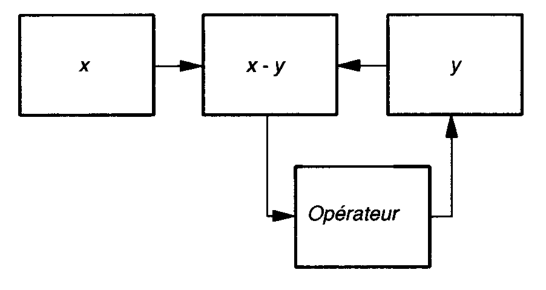
\includegraphics[width=8cm]{assets/figures/asscomp.pdf}
    \label{fig:asscomp}
\end{wrapfigure}
Les mesures par comparaison couvrent un très large nombre de mesures de toutes grandeurs. Le principe général est de comparer le mesurande $x$ à une grandeur connue de même nature $y$ pour obtenir $x=y$ ou $x-y=0$.

Cette grandeur de comparaison est parfois réglée par un opérateur - dont le rôle est celui d'un \textbf{asservissement} et peut être tenu par un dispositif automatique - qui agit sur $y$ pour obtenir que la valeur de $x-y$ formée par le \textbf{détecteur d'écart} soit nulle.

\subsubsection{A. méthode d'opposition ou méthode de zéro}

\begin{figure}[h]
    \centering
    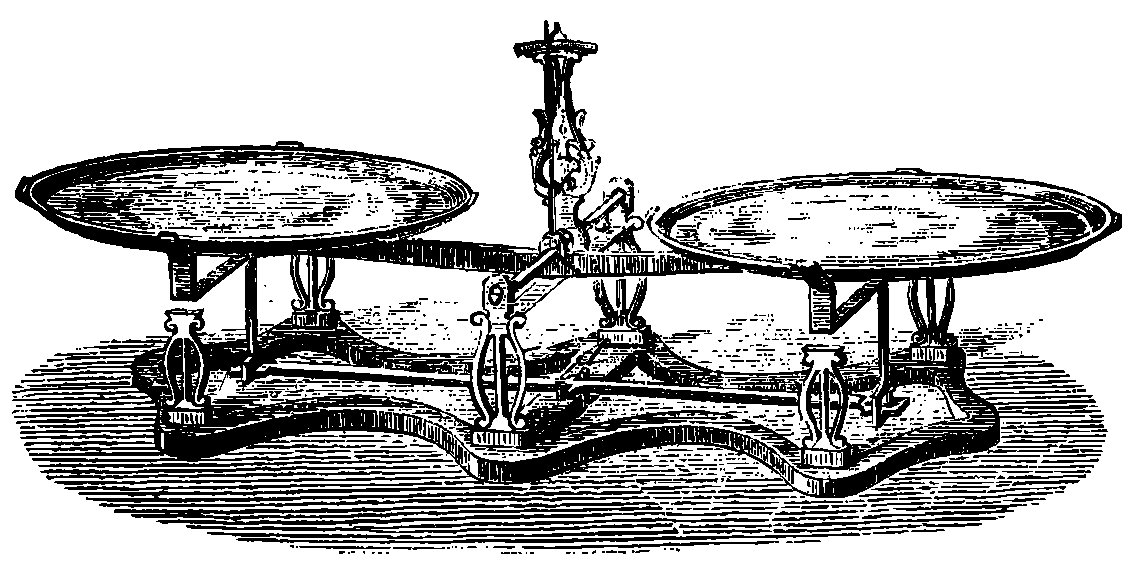
\includegraphics[height=4cm]{assets/figures/balande-roberval.pdf}\hspace{5mm}
    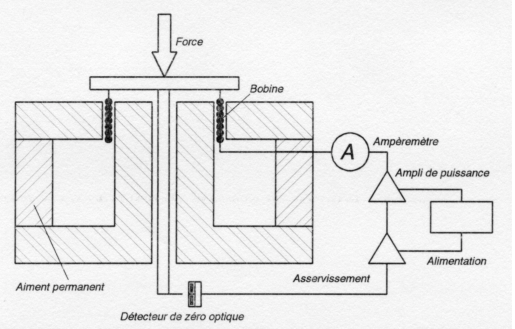
\includegraphics[height=4cm]{assets/figures/dynamo.pdf}
    \caption{Gauche: balance de Roberval. Droite: dynamomètre électromagnétique.}
    \label{fig:balance}
\end{figure}
Une \textbf{balance de Roberval} (figure \ref{fig:balance}) possède tous les organes d'un appareil de zéro: le soustracteur (fléau), le détecteur d'écart (l'aiguille), la grandeur d'opposition (boîte de poids). C'est l'opérateur qui apprécie l'écart puis dépose ou retire les poids pour obtenir l'équilibre.

Un autre exemple de méthode de zéro par asservissement est présenté en figure~\ref{fig:balance} (droite): il s'agit d'un \textbf{dynamomètre électromagnétique}. L'équilibre de la force présente sur le plateau est réalisé par une force électromagnétique grâce à un dispositif analogue à celui d'une bobine de haut-parleur. La commande électrique comprend le détecteur d'écart, la source d'énergie, l'amplificateur de puissance réglant l'intensité du courant, et un ampèremètre fournissant la valeur du poids.

\subsubsection{B. Montages en pont}

\begin{wrapfigure}[14]{l}[0pt]{6cm}
    \centering
    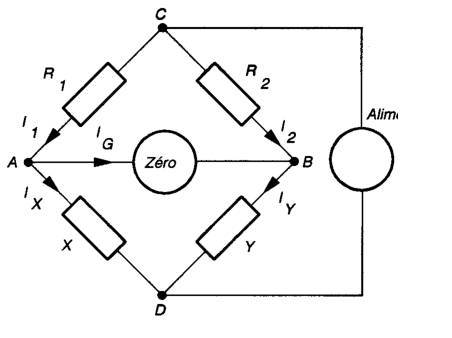
\includegraphics[width=6cm]{assets/figures/wheatstone.pdf}
    \caption{Pont de Wheatstone.}
    \label{fig:pont}
\end{wrapfigure}
Le montage en pont est un montage différentiel qui soustrait les réponses de deux bras contigus. Ceci permet de s'affranchir de l'influence de certaines grandeurs parasites qui pourraient masquer le phénomène auquel on porte intérêt.

Un pont est présenté traditionnellement comme un quadrilatère et deux connexions diagonales (AB et CD, figure \ref{fig:pont}). Les 4 côtés du quadrilatère constituent les bras. Une des diagonales (CD) contient l'alimentation en énergie; l'autre (AB) l'appareil de zéro. Lorsque la mesure d'une grandeur passive est faite par la méthode de déviation, les alimentations doivent avoir un niveau connu puisque la déviation leur est proportionnelle. Dans les montages en pont on est ramené en fait à la comparaison des valeurs des grandeurs passives qui constituent les bras, et par suite le niveau de l'unique source peut être quelconque à l'équilibre. L'application du \textbf{pont de Wheatstone} à la mesure des résistances électriques est bien connue (fig.~\ref{fig:pont}).

\subsubsection{C. méthode de déviation constante}

C'est encore une variante de la méthode de comparaison, mais ici la grandeur de comparaison conserve une valeur constante.  On ajoute au mesurande la quantité nécessaire pour atteindre la valeur fixée: x + y = constante. Cette méthode se retrouve en plusieurs variantes.

\subsubsection{D. méthode de la substitution}

Au mesurande on substitue une grandeur connue qui doit provoquer un effet identique. Puisqu'il s'agit de comparer deux effets successifs, il faut qu'un élément garde la trace du premier effet; il peut prendre dans certains appareils une place très importante, sous le nom de mémoire (figure \ref{fig:metsub}). Dans le cas du peson, par exemple, on décroche le poids inconnu et on le remplace par des poids marqués pour retrouver l'indication précédemment notée.
\begin{figure}[h]
    \centering
    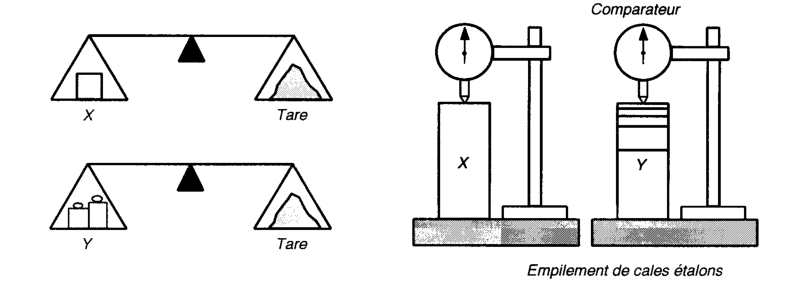
\includegraphics[width=15cm]{assets/figures/metsub.pdf}
    \caption{méthode de la substitution.}
    \label{fig:metsub}
\end{figure}

Pour une balance on fait l'équilibre avec une tare, puis on substitue des poids marqués à l'objet à peser. C'est la méthode dite de \textbf{Borda}. C'est la tare qui fait office de mémoire. La méthode s'étend à toutes sortes de mesures: différence de potentiel dans certains convertisseurs analogiques numériques, radioactivité, longueur, etc.

En contrôle dimensionnel, il est classique de substituer à la pièce dont la cote inconnue est gardée en mémoire sur un comparateur, un empilement de cales dont les dimensions sont bien connues, jusqu'à ramener le comparateur à la même indication.

\subsubsection{E. méthode de la permutation}

\begin{wrapfigure}[12]{r}[6pt]{6cm}
    \vspace{-2cm}
    \centering
    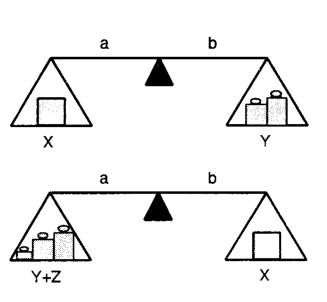
\includegraphics[width=6cm]{assets/figures/perm.pdf}
    \caption{méthode de la permutation.}
    \label{fig:perm}
\end{wrapfigure}
Lorsqu'on utilise un appareil qui réalise l'égalité $ax=by$, il faut en principe connaître $a/b$ pour avoir la mesure. Cependant, il est possible d'éliminer le facteur $a/b$ en effectuant deux mesures selon le schéma indiqué dans la figure \ref{fig:perm} : l'équilibre des moments donne
$$
    a\,x\,g=b\,y\,g\ \ \text{et}\ \ a\,(y+z)\,g=b\,x\,g
$$
et en divisant membre à membre on obtient
$$
    \frac{x}{y+z}=\frac{y}{x}
$$
soit finalement $x=\sqrt{y(y+z)}$. Appliquée aux balances à bras inégaux, cette méthode est connue sous le nom de méthode de \textbf{Gauss}.

\subsubsection{F. Appareils à seuil}

On se propose de connaître l'instant, ou les conditions, lorsque la grandeur x atteint une valeur prédéterminée. Ceci se rencontre en particulier lorsqu'on cherche à régler une variable à une valeur donnée (régulation), mais se rencontre aussi dans de nombreux processus métrologiques. La grandeur de comparaison a une valeur fixe et le détecteur de zéro se trouve bloqué par son action tant que le mesurande ne la surpasse pas. L'exemple typique en est les accéléromètres des airbags.

\subsection{Avantages et inconvénients des mesures par déviation et par comparaison}

Les caractères des mesures par déviation et par comparaison sont très différents. Le bilan sera dans l'ensemble favorable aux dernières, qui n'ont guère contre elles que leur relative complication et leur prix.

C'est le \textbf{détecteur d'écart} qui donne aux mesures par comparaison l'essentiel de leur caractère. L'absence d'exigences métrologiques à son égard, par opposition aux exigences formées pour les instruments de mesure par déviation, rend les mesures par comparaison plus précises que celles par déviation.

En effet, dans les méthodes par comparaison, le repérage de la position zéro est assuré par le détecteur d'écart qui fournit le \textbf{signal d'erreur} dont seuls l'existence et le signe nous intéressent. Ce fait permet de simplifier à l'extrême le détecteur sans exiger de lui des qualités métrologiques poussées. Il suffit que sa position d'équilibre soit stable, qu'il soit fidèle au zéro.

Dans tout instrument de mesure, la \textbf{justesse} est limitée par les défauts intrinsèques de l'instrument. Ces défauts se retrouvent évidemment aussi bien dans les mesures par déviation que dans les mesures par comparaison. Dans le cas des balances, l'influence des erreurs d'étalonnage, des erreurs sur les masses utilisées, des erreurs sur le parallélisme des couteaux, des erreurs sur les bras du fléau, etc. se retrouve dans les deux cas.

Il n'en va pas de même des \textbf{erreurs de lecture}. Dans la mesure par déviation, l'erreur de lecture représente en effet une fraction donnée de l'étendue de mesure, généralement de l'ordre de 1 à 0.1\%, alors que dans la méthode du zéro, la partie principale de la mesure porte sur des grandeurs connues avec exactitude, et leur somme ne peut être entachée d'aucune erreur (sauf de grossières erreurs, baptisées parasites par les normes, et qui sont en général faciles à dépister). L'erreur de lecture ne porte que sur l'évaluation du zéro, obtenue d'une manière précise par coïncidence. Pratiquement, elle est 100 à 1000 fois plus petite que l'erreur de la mesure par déviation.

Toutefois, l'usage de la méthode de déviation parait plus simple, donc plus prompt. Par exemple, un corps à peser est posé sur le plateau du peson à ressort et il suffit d'attendre un temps suffisant pour que l'élongation ait le temps de se stabiliser et que les oscillations soient amorties. Alors que la méthode de zéro suppose une série d'opérations qui comprennent la constatation d'un écart, l'application de la contre-réaction puis l'attente d'un nouvel équilibre.

Finalement, toute mesure consomme de l'énergie. Cependant il y a de ce point de vue une grande différence entre les méthodes de déviation et de comparaison. Dans le premier cas, l'énergie correspond à la déformation du système de mesure de sa position zéro à sa position d'équilibre final. Dans le second cas, elle ne correspond qu'à la déformation nécessaire pour observer l'écart.

Par exemple, si on évalue la tension d'une pile avec un voltmètre à cadre, il y a passage d'un courant tant que dure la mesure, et donc consommation d'énergie. Si au contraire on utilise la méthode d'opposition, aucun courant ne circule dans le galvanomètre de zéro et il n'y a aucune consommation d'énergie (donc aucune déformation du phénomène) autre que celle qui peut correspondre au plus petit écart discernable du galvanomètre. L'instrument de mesure se comporte comme s'il avait une impédance infinie.

\subsection{Comptages}

Il est très fréquent d'avoir à compter une certaine quantité d'éléments (nombre de tours, nombre d'impulsions, nombre de particules, etc.). La mesure se réduit alors à un comptage.

La fréquence de comptage des systèmes mécaniques ne dépasse pas quelques centaines de hertz; celle des compteurs électroniques dépasse 10 GHz.
